\subsection{Modelo de Ciclo de Vida do Software}

O software evolui. Modelo de Rajlich. Figura~\ref{fig:staged:model}. \textbf{Dimensão técnica.}

Na etapa de Desenvolvimento inicial (\textit{Initial development}) os desenvolvedores implementam a primeira versão funcional do software.
Se o desenvolvimento inicial for bem-sucedido, o software entra no estágio de Evolução (\textit{Evolution}), quando ocorrem mudanças iterativas, modificações e exclusões de funcionalidade. 
Na etapa de Serviço (\textit{Servicing}), os desenvolvedores fazem pequenos reparos de defeitos e mudanças funcionais simples.
Na etapa de \textit{Phaseout}, o software não recebe manutenção, mas continua disponível. No estágio de Fechamento (\textit{Closedown}), o software deixa de existir e seus usuários podem redirecionados para outro software, caso exista.

%Para o software de pesquisa, se existe um artigo de pesquisa que o utiliza, ...
%EXPLICAR que não há closedown... por causa da reprodutibilidade.
No contexto de desenvolvimento de software de pesquisa, é essencial considerar a continuidade e a reprodutibilidade do software ao longo do tempo, especialmente quando relacionado a artigos de pesquisa publicados.
Ao contrário de outros tipos de software, a etapa de Fechamento (\textit{Closedown}) não deve ser aplicada para permitir a reprodutibilidade dos resultados mencionados nos artigos.
Manter o software disponível e acessível é fundamental para que outros pesquisadores possam reproduzir e verificar os resultados obtidos.

\begin{figure}[htb]
    \centering
    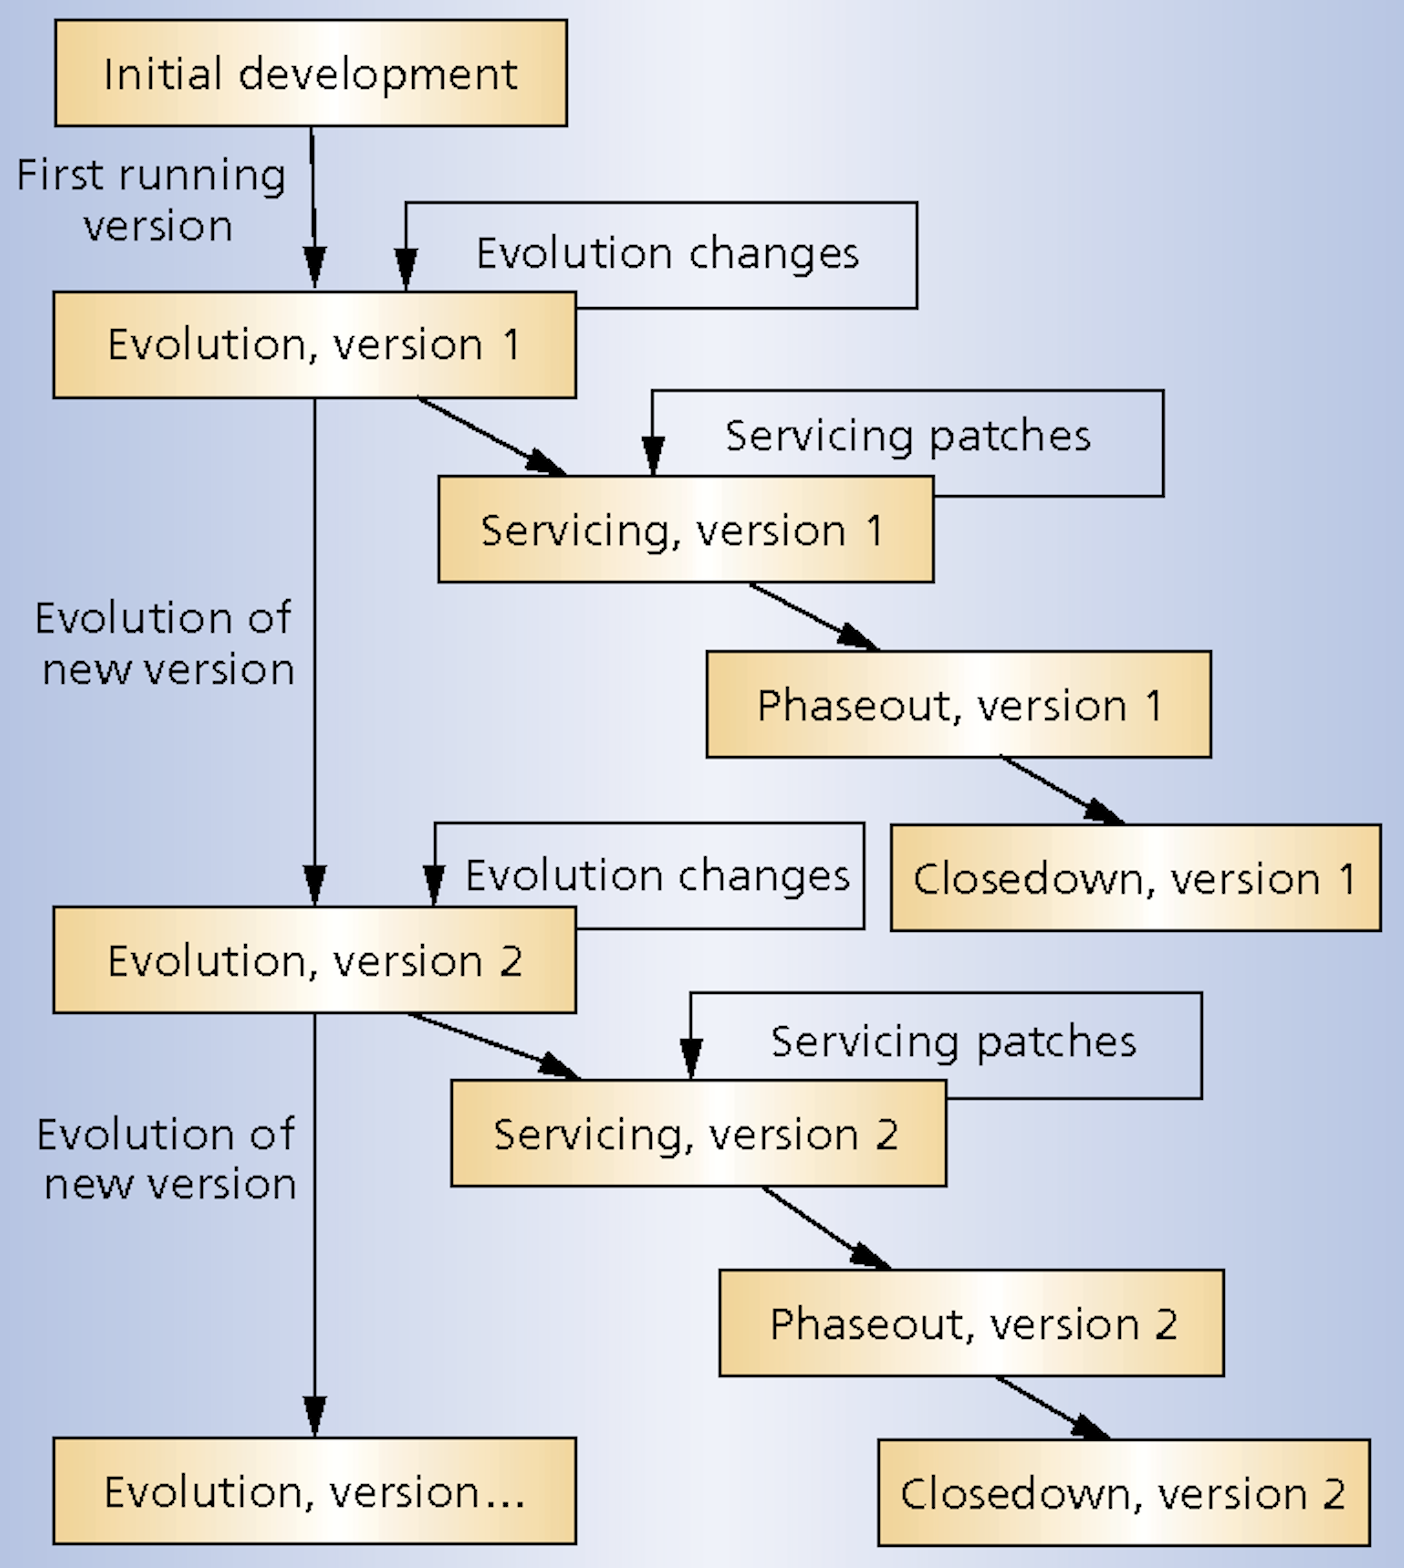
\includegraphics[scale=0.35]{JAI 2023/figures/staged-model-versions.png}
    \caption{Original~\cite{rajlich:staged:2000} \textit{A versioned staged model for the software life cycle emphasizes the evolutionary nature of software development.}}
    \label{fig:staged:model}
\end{figure}

O modelo de Rajlich destaca que, em determinados intervalos, uma versão do software é liberada para a comunidade. 

\textbf{Dimensão social.} 

A estrutura do grupo de pesquisa envolvido no desenvolvimento do software de pesquisa pode se refletir na estrutura do projeto ... 
A pesquisa evolui, o grupo de pesquisa recebe novos membros, o software evolui, novo software pode ser criado que interfaceia com outros ...


Holland: Many software maintenance problems are not technical but people problems. 
We need to be able to organize the development team (group, community, etc.) in such a way that it embraces change and facilitates maintenance and evolution, not only immediately after deployment of the software, but for the decades that follow.

- Abrir para contribuição externa?


